\documentclass[11pt,a4paper]{article}

% ---------------------------------------------------------------------------
% CyberRange OS - Project Documentation
% Compile with: pdflatex CyberRangeOS.tex  (run twice for the ToC)
% Pure LaTeX + TikZ; no external images required.
% ---------------------------------------------------------------------------

\usepackage[margin=2.2cm]{geometry}
\usepackage[T1]{fontenc}
\usepackage{lmodern}
\usepackage{xcolor}
\usepackage{graphicx}
\usepackage{booktabs}
\usepackage{enumitem}
\usepackage{titlesec}
\usepackage{fancyhdr}
\usepackage{listings}
\usepackage{tikz}
\usepackage{amssymb}
\usepackage[hidelinks]{hyperref}
\usetikzlibrary{shapes.geometric, arrows.meta, positioning, fit, backgrounds, calc}

% ------------------------------------------------------------------ palette
\definecolor{vblack}{HTML}{0A0A0B}
\definecolor{vsoft}{HTML}{17171A}
\definecolor{vwhite}{HTML}{F5F3EE}
\definecolor{vgold}{HTML}{D4AF37}
\definecolor{vred}{HTML}{C41E3A}
\definecolor{vreddeep}{HTML}{8B0000}
\definecolor{vslate}{HTML}{2E3440}
\definecolor{vgoldbright}{HTML}{F4CD5C}
\definecolor{codebg}{HTML}{F4F2EC}

\hypersetup{colorlinks=true, linkcolor=vreddeep, urlcolor=vreddeep, citecolor=vreddeep}

% ------------------------------------------------------------------ headers
\pagestyle{fancy}
\fancyhf{}
\lhead{\textsc{CyberRange OS}}
\rhead{\thepage}
\lfoot{\small AI-Augmented Red/Blue Team Training Platform}
\rfoot{\small Confidential --- Institution Use}
\renewcommand{\headrulewidth}{0.5pt}
\renewcommand{\footrulewidth}{0.3pt}

\titleformat{\section}{\Large\bfseries\color{vreddeep}}{\thesection}{0.6em}{}
\titleformat{\subsection}{\large\bfseries\color{vslate}}{\thesubsection}{0.6em}{}

% ------------------------------------------------------------------ listings
\lstset{
  basicstyle=\ttfamily\small,
  backgroundcolor=\color{codebg},
  breaklines=true,
  frame=single,
  rulecolor=\color{vslate},
  numbers=none,
  columns=fullflexible,
  keepspaces=true,
  showstringspaces=false,
  captionpos=b
}

% ------------------------------------------------------------------ tikz styles
\tikzset{
  box/.style={rectangle, rounded corners=2pt, draw=vslate, fill=vsoft, text=vwhite,
              minimum height=0.9cm, minimum width=2.6cm, align=center, font=\small},
  gold/.style={draw=vgold, fill=vblack, text=vgold},
  red/.style={draw=vred, fill=vblack, text=vred},
  store/.style={cylinder, shape border rotate=90, aspect=0.3, draw=vslate, fill=vsoft,
                text=vwhite, minimum height=1.1cm, minimum width=2.2cm, align=center, font=\small},
  flow/.style={-{Stealth[length=2.2mm]}, draw=vslate, thick},
  goldflow/.style={-{Stealth[length=2.2mm]}, draw=vgold, thick},
  redflow/.style={-{Stealth[length=2.2mm]}, draw=vred, thick},
  wstep/.style={rectangle, rounded corners=3pt, draw=vgold, fill=vsoft, text=vwhite,
               minimum height=1.0cm, text width=3.1cm, align=center, font=\small\sffamily}
}
\setlength{\headheight}{14pt}

\begin{document}

% ============================================================ TITLE PAGE
\begin{titlepage}
\centering
\vspace*{1.2cm}
{\Huge\bfseries\color{vreddeep} CyberRange OS\par}
\vspace{0.4cm}
{\Large AI-Augmented Red Team / Blue Team Training Platform\par}
\vspace{0.2cm}
{\large\itshape Self-hosted, locally-inferenced, accreditation-ready\par}
\vspace{1.4cm}


\begin{tikzpicture}
  \node[gold, box, minimum width=8cm, minimum height=1.4cm] (t)
    {\textbf{Department Cybersecurity Lab}\\ \small NBA/NAAC-aligned $\cdot$ Locally hosted LLMs};
\end{tikzpicture}

\vspace{1.6cm}
\begin{tabular}{rl}
\textbf{Document} & Project Design \& Implementation Report\\
\textbf{Scope} & Requirements, Architecture, Implementation, Deployment\\
\textbf{Backend} & Go 1.25 + Fiber\\
\textbf{Frontend} & Next.js 14 (App Router) + TypeScript + Tailwind\\
\textbf{Local LLM} & Ollama / vLLM / TGI (open-weight models)\\
\textbf{Repository} & \texttt{github.com/MD-HACKER07/CyberRange-OS}\\
\end{tabular}

\vfill
{\small Every LLM call goes to a private endpoint; no student data, lab logs, or
exploit attempts leave the institution's network.\par}
\vspace{0.6cm}
{\small \today\par}
\end{titlepage}

\tableofcontents
\newpage

% ============================================================ 1. OVERVIEW
\section{Executive Summary}
CyberRange OS is a self-hosted web platform that lets cybersecurity students
practice, under supervision, both \textbf{offensive} security (reconnaissance,
exploitation, reporting against an isolated, intentionally-vulnerable target
range) and \textbf{defensive} security (log analysis, threat detection, incident
response) through a real SOC-style workflow. Every exercise is assisted by a
\textbf{locally-hosted, open-weight LLM}, so no student data, lab logs, or
exploit attempts ever leave the institution's network.

The platform produces structured evidence --- attempt logs, scores,
rubric-graded reports, and time-to-detect metrics --- that maps to Course
Outcomes (CO) and Programme Outcomes (PO) for \textbf{NBA} accreditation, and
aggregates research/innovation evidence for \textbf{NAAC}.

\subsection{Roles Served}
\begin{itemize}[leftmargin=*]
  \item \textbf{Student} --- enroll in batches, run Red/Blue exercises, submit reports, view CO/PO progress and leaderboard rank.
  \item \textbf{Faculty/Instructor} --- author exercises with rubrics, map to CO/PO, grade reports (override AI suggestions), view class dashboards.
  \item \textbf{Lab Admin} --- provision range targets, manage the LLM model registry and prompts, manage users/RBAC, view the full audit log.
  \item \textbf{Auditor (read-only)} --- view aggregated CO/PO/NAAC evidence exports only.
\end{itemize}

% ============================================================ 2. WHAT IT CAN DO
\section{Capabilities --- What the Platform Can Do}

\begin{table}[h]
\centering
\small
\begin{tabular}{@{}p{4.2cm}p{10.5cm}@{}}
\toprule
\textbf{Module} & \textbf{Capability}\\
\midrule
Auth \& Identity & JWT access + rotating refresh tokens, institution SSO (OIDC) with local fallback, four RBAC roles, append-only audit trail.\\
Red Team Range & Per-session isolated range provisioning, browser-driven command execution in a Kali container, full command logging, LLM pentest copilot (suggest $\rightarrow$ approve $\rightarrow$ execute), MITRE auto-tagging, live resource stats, tool quick-actions.\\
LLM Gateway & Local-inference-only guard, model registry, versioned system prompts, streaming, per-session token budgets, complete prompt/completion logging for reproducibility.\\
Blue Team SOC & Wazuh + Suricata ingestion into a common alert schema, live alert console with severity filters, SOC copilot (summary/verdict/next-step), MTTD/MTTR timers, playbooks, faculty ground-truth labeling, accuracy dashboard.\\
MITRE ATT\&CK Engine & STIX/curated dataset ingest, pgvector semantic search, LLM disambiguation, per-session technique tracker.\\
Reporting Engine & Markdown editor with live preview, AI grading assistant (faculty authoritative), PDF export, combined portfolio PDF.\\
Accreditation Analytics & CO/PO matrix, weighted direct/indirect attainment, heatmap, NBA CSV \& NAAC evidence exports, course-exit surveys.\\
AI Security & PyRIT/Garak (or built-in probe battery) run against the institution's own local model; results dashboard.\\
Gamification & XP weighted by difficulty and inverse copilot reliance; red/blue/combined leaderboards; pluggable external CTF feed.\\
Voice Assistant & Real-time speech Q\&A about department routine and platform usage, answered by the local model, with an admin-editable knowledge base.\\
Admin \& Observability & Range target provisioning, LLM registry, RBAC, audit viewer with CSV export, system health, Prometheus metrics.\\
\bottomrule
\end{tabular}
\caption{Functional capability matrix.}
\end{table}

% ============================================================ 3. ARCHITECTURE
\section{System Architecture}
CyberRange OS is a service-oriented, on-prem monorepo. The Go API is a modular
monolith --- one deployable binary containing the auth, orchestrator, LLM
gateway, log-ingest, MITRE, analytics, reporting, and AI-security subsystems ---
each behind a clean interface so it can later be split into its own process.

\begin{figure}[h]
\centering
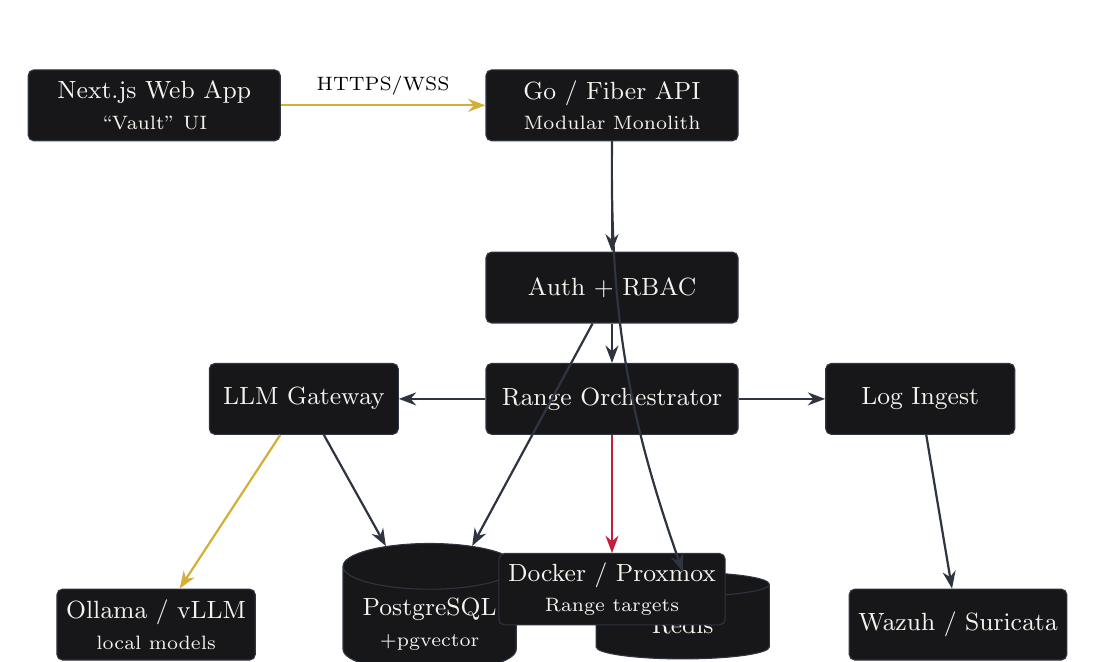
\begin{tikzpicture}[node distance=0.9cm and 1.1cm]
  \node[gold, box, minimum width=3.2cm] (web) {Next.js Web App\\\scriptsize ``Vault'' UI};
  \node[gold, box, minimum width=3.2cm, right=2.6cm of web] (api) {Go / Fiber API\\\scriptsize Modular Monolith};
  \node[box, below=1.4cm of api, minimum width=3.2cm] (auth) {Auth + RBAC};
  \node[red, box, below=0.5cm of auth, minimum width=3.2cm] (orch) {Range Orchestrator};
  \node[box, left=1.1cm of orch, minimum width=2.4cm] (llm) {LLM Gateway};
  \node[box, right=1.1cm of orch, minimum width=2.4cm] (ingest) {Log Ingest};

  \node[store, below left=1.5cm and -0.2cm of orch] (pg) {PostgreSQL\\\scriptsize +pgvector};
  \node[store, right=1.0cm of pg] (redis) {Redis};
  \node[red, box, below=1.5cm of orch, minimum width=2.6cm] (docker) {Docker / Proxmox\\\scriptsize Range targets};
  \node[gold, box, left=1.1cm of pg, minimum width=2.4cm] (ollama) {Ollama / vLLM\\\scriptsize local models};
  \node[box, right=1.0cm of redis, minimum width=2.4cm] (siem) {Wazuh / Suricata};

  \draw[goldflow] (web) -- node[above,font=\scriptsize]{HTTPS/WSS} (api);
  \draw[flow] (api) -- (auth);
  \draw[flow] (auth) -- (orch);
  \draw[flow] (orch) -- (llm);
  \draw[flow] (orch) -- (ingest);
  \draw[flow] (auth) -- (pg);
  \draw[flow] (api.south) to[bend right=10] (redis.north);
  \draw[redflow] (orch) -- (docker);
  \draw[goldflow] (llm) -- (ollama);
  \draw[flow] (ingest) -- (siem);
  \draw[flow] (llm) -- (pg);
\end{tikzpicture}
\caption{High-level architecture. Gold = brand/LLM paths, red = Red Team range paths.}
\end{figure}

\subsection{Backend Packages (\texttt{apps/api/internal})}
\begin{table}[h]
\centering
\small
\begin{tabular}{@{}ll@{}}
\toprule
\textbf{Package} & \textbf{Responsibility}\\
\midrule
\texttt{config} & Env-driven configuration; every dependency is a configurable URL.\\
\texttt{auth} & JWT access/refresh (rotating), OIDC SSO, local password, RBAC middleware.\\
\texttt{audit} & Append-only audit trail (DB trigger blocks UPDATE/DELETE).\\
\texttt{llm} & Local-inference gateway: egress guard, model registry, versioned prompts, streaming, budgets, call logging.\\
\texttt{orchestrator} & \texttt{RangeProvisioner} interface + \texttt{DockerDriver} and \texttt{ProxmoxDriver}.\\
\texttt{ingest} & Polls Wazuh REST + tails Suricata EVE JSON into the common Alert schema.\\
\texttt{mitre} & ATT\&CK dataset, pgvector semantic search, LLM auto-tagging.\\
\texttt{report} & Markdown $\rightarrow$ HTML $\rightarrow$ PDF rendering.\\
\texttt{aisec} & PyRIT/Garak runner against the local model (built-in probe fallback).\\
\texttt{store} & Data access for courses, batches, exercises, sessions, reports, analytics.\\
\texttt{server} & Fiber wiring + per-module HTTP/WS handlers.\\
\bottomrule
\end{tabular}
\caption{Backend module responsibilities.}
\end{table}

% ============================================================ 4. NETWORK ISOLATION
\section{Network Isolation \& Safety Model}
The range is structurally prevented from touching arbitrary hosts: attack
targets are selected only from a pre-registered dropdown of range assets --- no
free-text host field exists anywhere. Range networks are provisioned with the
Docker \texttt{internal:true} flag, so Docker attaches \emph{no gateway to the
WAN}.

\begin{figure}[h]
\centering
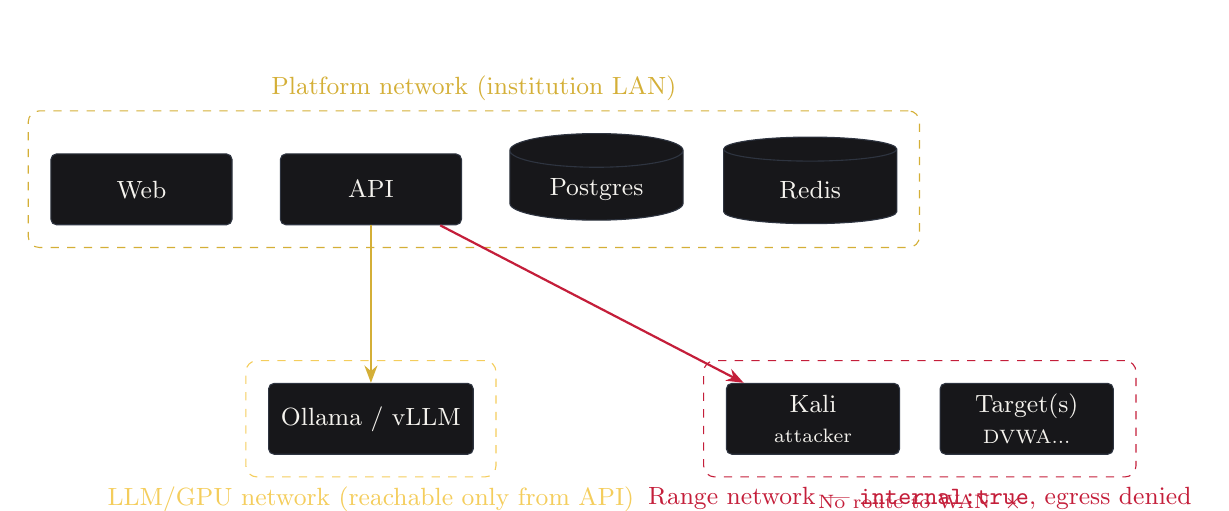
\begin{tikzpicture}[node distance=0.8cm]
  % platform network
  \node[gold, box, minimum width=2.3cm] (web) {Web};
  \node[gold, box, right=0.6cm of web, minimum width=2.3cm] (api) {API};
  \node[store, right=0.6cm of api] (db) {Postgres};
  \node[store, right=0.5cm of db] (rd) {Redis};
  \begin{scope}[on background layer]
    \node[draw=vgold, dashed, rounded corners, fit=(web)(api)(db)(rd),
          inner sep=8pt, label={[vgold]above:\small Platform network (institution LAN)}] (plat) {};
  \end{scope}

  % LLM network
  \node[gold, box, below=2.0cm of api, minimum width=2.6cm] (oll) {Ollama / vLLM};
  \begin{scope}[on background layer]
    \node[draw=vgoldbright, dashed, rounded corners, fit=(oll), inner sep=8pt,
          label={[vgoldbright]below:\small LLM/GPU network (reachable only from API)}] (llmn) {};
  \end{scope}

  % range network
  \node[red, box, right=3.2cm of oll, minimum width=2.2cm] (kali) {Kali\\\scriptsize attacker};
  \node[red, box, right=0.5cm of kali, minimum width=2.2cm] (tgt) {Target(s)\\\scriptsize DVWA...};
  \begin{scope}[on background layer]
    \node[draw=vred, dashed, rounded corners, fit=(kali)(tgt), inner sep=8pt,
          label={[vred]below:\small Range network --- \texttt{internal:true}, egress denied}] (rangen) {};
  \end{scope}

  \draw[goldflow] (api) -- (oll);
  \draw[redflow] (api) -- (kali);
  \node[below=0.1cm of rangen, vred, font=\scriptsize] {No route to WAN $\;\times$};
\end{tikzpicture}
\caption{Three logical networks. Range traffic cannot reach the internet.}
\end{figure}

\subsection{Non-Negotiable Guardrails}
\begin{enumerate}[leftmargin=*]
  \item Targets come only from the \texttt{range\_targets} registry (dropdown), never free text.
  \item The copilot never auto-executes; a human clicks \textbf{Approve \& Run}, and every approved action is logged with student, target, timestamp, and full command.
  \item All LLM traffic goes to \texttt{LLM\_BASE\_URL}; the gateway refuses to start if that resolves to a public IP (unless explicitly overridden for a lab-controlled network).
  \item The audit log is append-only, enforced by a database trigger.
\end{enumerate}

% ============================================================ 5. RED TEAM FLOW
\section{Red Team Workflow}
\begin{figure}[h]
\centering
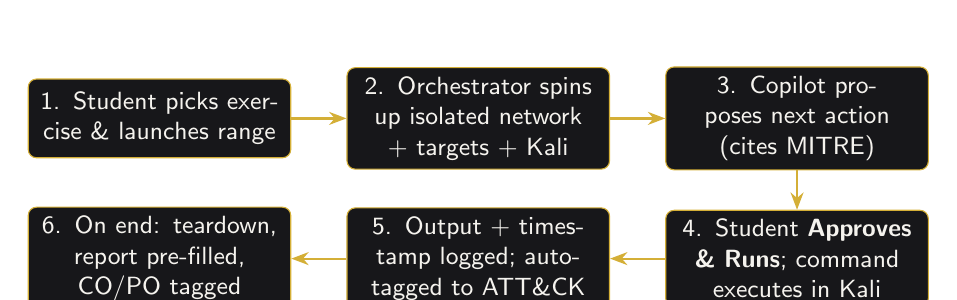
\begin{tikzpicture}[node distance=0.5cm and 0.7cm]
  \node[wstep] (s1) {1. Student picks exercise \& launches range};
  \node[wstep, right=of s1] (s2) {2. Orchestrator spins up isolated network + targets + Kali};
  \node[wstep, right=of s2] (s3) {3. Copilot proposes next action (cites MITRE)};
  \node[wstep, below=of s3] (s4) {4. Student \textbf{Approves \& Runs}; command executes in Kali};
  \node[wstep, left=of s4] (s5) {5. Output + timestamp logged; auto-tagged to ATT\&CK};
  \node[wstep, left=of s5] (s6) {6. On end: teardown, report pre-filled, CO/PO tagged};

  \draw[goldflow] (s1) -- (s2);
  \draw[goldflow] (s2) -- (s3);
  \draw[goldflow] (s3) -- (s4);
  \draw[goldflow] (s4) -- (s5);
  \draw[goldflow] (s5) -- (s6);
\end{tikzpicture}
\caption{Human-in-the-loop Red Team session lifecycle.}
\end{figure}

The primary evidence artifact is the \texttt{session\_command\_log} table: every
executed command, its captured output, exit code, whether it was AI-suggested,
and the mapped ATT\&CK technique. Copilot \emph{suggestions} are stored even when
never approved, proving human-in-the-loop control.

% ============================================================ 6. BLUE TEAM FLOW
\section{Blue Team Workflow}
\begin{figure}[h]
\centering
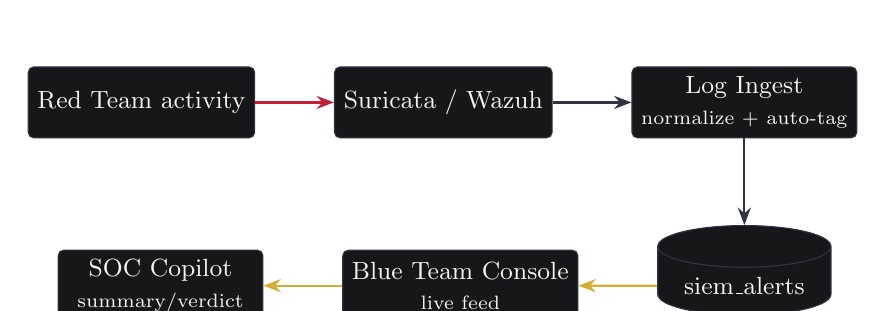
\begin{tikzpicture}[node distance=0.9cm and 1.0cm]
  \node[red, box, minimum width=2.6cm] (attack) {Red Team activity};
  \node[box, right=of attack, minimum width=2.6cm] (ids) {Suricata / Wazuh};
  \node[box, right=of ids, minimum width=2.6cm] (ing) {Log Ingest\\\scriptsize normalize + auto-tag};
  \node[store, below=1.1cm of ing] (pg) {siem\_alerts};
  \node[gold, box, left=of pg, minimum width=2.6cm] (console) {Blue Team Console\\\scriptsize live feed};
  \node[gold, box, left=of console, minimum width=2.6cm] (copilot) {SOC Copilot\\\scriptsize summary/verdict};

  \draw[redflow] (attack) -- (ids);
  \draw[flow] (ids) -- (ing);
  \draw[flow] (ing) -- (pg);
  \draw[goldflow] (pg) -- (console);
  \draw[goldflow] (console) -- (copilot);
\end{tikzpicture}
\caption{Real telemetry pipeline: attacks generate IDS events that students triage live.}
\end{figure}

MTTD (mean time to detect) starts when the paired Red Team action occurs; MTTR
(mean time to respond) stops when the student marks the alert resolved with a
written response. Faculty set the ground-truth label per alert, so the platform
measures both \textbf{copilot accuracy} and \textbf{student accuracy} against
ground truth (a CyberSOCEval-style comparison).

% ============================================================ 7. DATA MODEL
\section{Core Data Model}
\begin{figure}[h]
\centering
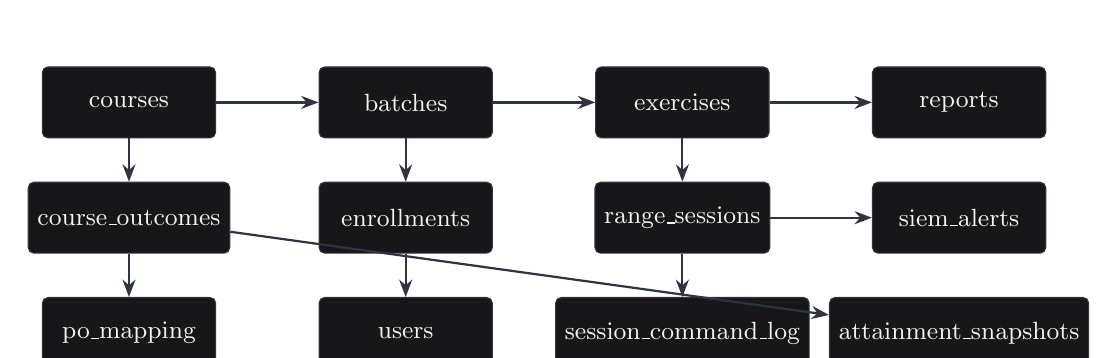
\begin{tikzpicture}[node distance=0.55cm and 1.3cm, every node/.style={font=\scriptsize}]
  \node[box, minimum width=2.2cm] (course) {courses};
  \node[box, below=of course, minimum width=2.2cm] (co) {course\_outcomes};
  \node[box, below=of co, minimum width=2.2cm] (po) {po\_mapping};
  \node[box, right=of course, minimum width=2.2cm] (batch) {batches};
  \node[box, below=of batch, minimum width=2.2cm] (enr) {enrollments};
  \node[box, below=of enr, minimum width=2.2cm] (user) {users};
  \node[box, right=of batch, minimum width=2.2cm] (ex) {exercises};
  \node[box, below=of ex, minimum width=2.2cm] (sess) {range\_sessions};
  \node[box, below=of sess, minimum width=2.2cm] (clog) {session\_command\_log};
  \node[box, right=of ex, minimum width=2.2cm] (rep) {reports};
  \node[box, below=of rep, minimum width=2.2cm] (alert) {siem\_alerts};
  \node[box, below=of alert, minimum width=2.2cm] (att) {attainment\_snapshots};

  \draw[flow] (course) -- (co);
  \draw[flow] (co) -- (po);
  \draw[flow] (course) -- (batch);
  \draw[flow] (batch) -- (enr);
  \draw[flow] (enr) -- (user);
  \draw[flow] (batch) -- (ex);
  \draw[flow] (ex) -- (sess);
  \draw[flow] (sess) -- (clog);
  \draw[flow] (ex) -- (rep);
  \draw[flow] (sess) -- (alert);
  \draw[flow] (co) -- (att);
\end{tikzpicture}
\caption{Selected core tables and relationships (full schema in \texttt{0001\_init.sql}).}
\end{figure}

Additional tables include \texttt{llm\_prompts} (versioned), \texttt{llm\_calls}
(full input/output logging), \texttt{copilot\_suggestions}, \texttt{playbooks},
\texttt{ai\_redteam\_scans}, \texttt{leaderboard\_entries}, \texttt{surveys}, and
\texttt{audit\_log}.

% ============================================================ 8. TECH STACK
\section{Technology Stack}
\begin{table}[h]
\centering
\small
\begin{tabular}{@{}ll@{}}
\toprule
\textbf{Layer} & \textbf{Technology}\\
\midrule
Backend API & Go 1.25 + Fiber v2\\
Frontend & Next.js 14 (App Router), TypeScript, Tailwind CSS\\
Realtime & WebSockets via Redis pub/sub fan-out\\
Primary DB & PostgreSQL 16 with pgvector\\
Cache / Queue / Pub-Sub & Redis 7\\
Auth & JWT (access + rotating refresh), OIDC SSO, local fallback\\
Local LLM runtime & Ollama (dev) / vLLM (prod) --- open-weight models\\
Range orchestration & Docker Engine API (\texttt{DockerDriver}); Proxmox driver stub\\
SIEM / IDS & Wazuh manager + Suricata (EVE JSON)\\
Offensive tooling & Kali container: nmap, Metasploit, sqlmap, gobuster, nikto, hydra\\
AI red-teaming & PyRIT / Garak against the local model\\
Reporting & Headless Chromium / wkhtmltopdf for PDF\\
Observability & Prometheus metrics + structured JSON logging (zerolog)\\
\bottomrule
\end{tabular}
\caption{Technology choices per layer.}
\end{table}

% ============================================================ 9. LLM GATEWAY
\section{Local LLM Gateway --- ``No Data Leaves'' Guarantee}
All modules call through a single gateway; nothing in the frontend talks to
the model directly. The gateway enforces the local-inference guarantee at
startup:

\begin{lstlisting}[language=Go, caption={Egress guard (simplified).}]
func AssertLocalEndpoint(rawURL string, allowPublic bool) (*EgressAssertion, error) {
    // resolve host -> IPs; every IP must be loopback/private (RFC1918, CGNAT).
    // If any resolves to a public address and the override is off, refuse to start.
}
\end{lstlisting}

Per-module system prompts are stored in the database and versioned; every call
records the model and prompt version used, so graded work stays reproducible for
accreditation review. Modules: \texttt{pentest-copilot}, \texttt{soc-copilot},
\texttt{report-grading}, \texttt{mitre-tagging}, \texttt{red-teaming-target}, and
\texttt{assistant}.

% ============================================================ 10. VOICE ASSISTANT
\section{Real-Time Voice Department Assistant}
Students and faculty can ask --- by voice or text --- about department routine,
timings, contacts, rules, or how to use the platform. Speech-to-text and
text-to-speech run in the browser (Web Speech API); the \emph{answer} is
generated by the local model, so knowledge stays on-prem. Faculty/admin edit a
knowledge base that grounds the answers; the assistant is instructed not to
invent facts it does not have.

% ============================================================ 11. ACCREDITATION
\section{Accreditation Analytics (CO/PO, NBA/NAAC)}
Each graded exercise contributes an attainment data point per tagged CO. The
platform computes the standard weighted direct/indirect attainment
(configurable, e.g. 80/20), rolls it up to POs via the mapping matrix, and
renders a heatmap. Exports include an NBA-format attainment CSV per batch and a
NAAC evidence summary (student projects, AI-security findings, range usage).

\[
\text{CO}_{\text{final}} = w_d \cdot \text{Direct}\% + w_i \cdot \text{Indirect}\%,
\qquad
\text{PO}_{\text{score}} = \frac{\sum_i \text{CO}_i \cdot \text{weight}_i}{\sum_i \text{weight}_i}
\]

% ============================================================ 12. DEPLOYMENT
\section{Deployment}
\begin{figure}[h]
\centering
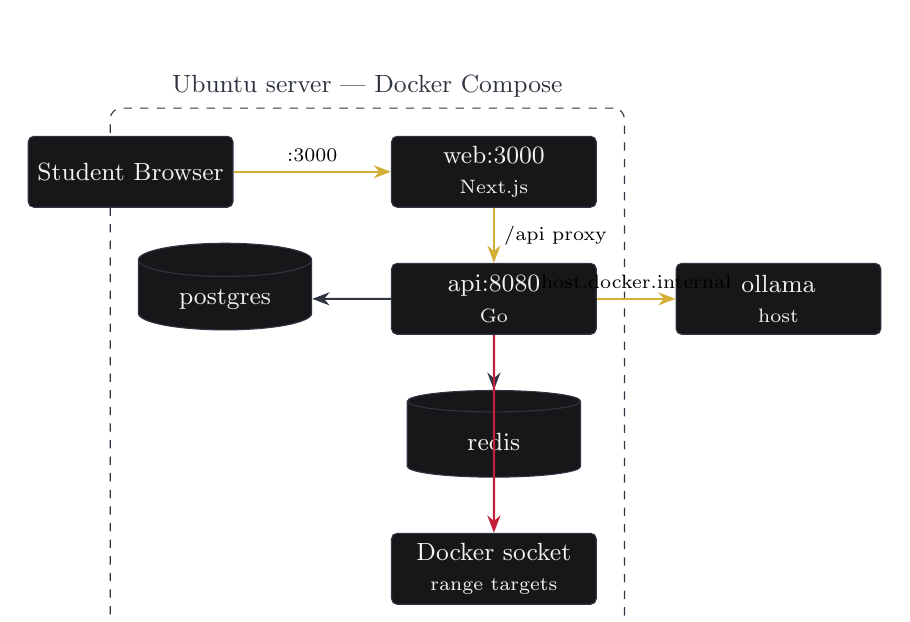
\begin{tikzpicture}[node distance=0.7cm and 1.0cm]
  \node[gold, box] (browser) {Student Browser};
  \node[gold, box, right=2.0cm of browser] (web) {web:3000\\\scriptsize Next.js};
  \node[gold, box, below=of web] (api) {api:8080\\\scriptsize Go};
  \node[store, left=of api] (pg) {postgres};
  \node[store, below=of api] (redis) {redis};
  \node[gold, box, right=of api] (oll) {ollama\\\scriptsize host};
  \node[red, box, below=of redis] (dock) {Docker socket\\\scriptsize range targets};

  \draw[goldflow] (browser) -- node[above,font=\scriptsize]{:3000} (web);
  \draw[goldflow] (web) -- node[right,font=\scriptsize]{/api proxy} (api);
  \draw[flow] (api) -- (pg);
  \draw[flow] (api) -- (redis);
  \draw[goldflow] (api) -- node[above,font=\scriptsize]{host.docker.internal} (oll);
  \draw[redflow] (api) -- (dock);
  \begin{scope}[on background layer]
    \node[draw=vslate, dashed, rounded corners, fit=(web)(api)(pg)(redis)(dock),
          inner sep=10pt, label={[vslate]above:\small Ubuntu server --- Docker Compose}] {};
  \end{scope}
\end{tikzpicture}
\caption{Single-server deployment (\texttt{docker-compose.deploy.yml}). Native Ollama reused via the private Docker bridge.}
\end{figure}

\begin{lstlisting}[language=bash, caption={One-command server bring-up.}]
git clone git@github.com:MD-HACKER07/CyberRange-OS.git && cd CyberRange-OS
cp .env.deploy.example .env.deploy   # set POSTGRES_PASSWORD, JWT_SECRET, admin pass
docker build -t cyberrange/kali-attacker:latest infra/kali
docker compose -f infra/docker-compose.deploy.yml --env-file .env.deploy up -d --build
\end{lstlisting}

% ============================================================ 13. WHAT WE BUILT
\section{Implementation Status --- What We Built}
\begin{table}[h]
\centering
\small
\begin{tabular}{@{}p{5.2cm}p{3.0cm}p{6.0cm}@{}}
\toprule
\textbf{Component} & \textbf{Status} & \textbf{Notes}\\
\midrule
Auth, RBAC, audit trail & \textbf{Done} & JWT rotation, OIDC, 4 roles, append-only log.\\
Courses/batches/exercises CRUD & \textbf{Done} & Faculty authoring, publish workflow.\\
Range orchestrator (Docker) & \textbf{Done} & Isolated networks, exec, teardown, stats.\\
Proxmox driver & \textbf{Interface stub} & Same interface, ready for completion.\\
LLM Gateway + egress guard & \textbf{Done} & Model registry, versioned prompts, budgets, logging.\\
Red Team console & \textbf{Done} & Live terminal, copilot approve/run, tool palette, ATT\&CK tracker.\\
Blue Team console & \textbf{Done} & Alert feed, SOC copilot, MTTD/MTTR, filters, ground-truth.\\
Log ingest (Wazuh + Suricata) & \textbf{Done} & Common schema, auto-tag, live stream.\\
MITRE engine & \textbf{Done} & Curated + STIX ingest, pgvector semantic search.\\
Reporting + PDF & \textbf{Done} & Editor, AI grade, portfolio export.\\
Accreditation analytics & \textbf{Done} & CO/PO attainment, heatmap, NBA/NAAC exports, surveys.\\
AI Security (PyRIT/Garak) & \textbf{Done} & CLI integration + built-in probe fallback.\\
Gamification \& leaderboards & \textbf{Done} & XP with assistance ratio, tracks.\\
Voice assistant & \textbf{Done} & Local-LLM Q\&A + editable knowledge base.\\
Demo content seed & \textbf{Done} & Course, faculty+student, 3 exercises, playbook.\\
Docker Compose deployment & \textbf{Done} & Single-server compose + Suricata profile.\\
\bottomrule
\end{tabular}
\caption{Build status across all phases (1--10 plus enhancements).}
\end{table}

\subsection{Verification}
The Go backend compiles cleanly and passes unit tests (including the egress-guard
suite). The Next.js frontend type-checks and builds all 17 routes. The full
stack has been run end-to-end: database migrations and reference-data seeding,
admin login, and a live connection to a local Ollama model serving
\texttt{llama3.2:3b} and \texttt{nomic-embed-text}.

% ============================================================ 14. USAGE
\section{How Students \& Faculty Use It}
\begin{enumerate}[leftmargin=*]
  \item \textbf{Log in} with college email/roll number (SSO or local).
  \item \textbf{Dashboard}: batch, active session card, CO/PO progress, leaderboard snippet.
  \item \textbf{Red Team}: choose a published exercise, launch the range, run recon/exploit commands, approve copilot suggestions; every action is logged and MITRE-tagged.
  \item \textbf{Blue Team}: triage live alerts with the SOC copilot, resolve with a written note; MTTD/MTTR tracked.
  \item \textbf{Reports}: write and submit a pentest/incident report (auto-seeded from the session timeline), export PDF, build a portfolio.
  \item \textbf{Assistant / Learning Paths / Leaderboard}: ask questions by voice, track certification coverage and XP.
  \item \textbf{Faculty}: author exercises, grade with rubric (override AI), set alert ground truth, view CO/PO heatmap and SOC accuracy, export NBA/NAAC evidence.
\end{enumerate}

% ============================================================ 15. FUTURE
\section{Roadmap / What We Can Do Next}
\begin{itemize}[leftmargin=*]
  \item Complete the \textbf{Proxmox driver} for full VM-level isolation in production.
  \item Add \textbf{browser desktop} access (Apache Guacamole) for GUI tools like Burp Suite.
  \item Offline \textbf{Whisper} service for fully-local speech-to-text.
  \item TLS on the Docker Engine API and mutual-TLS between services.
  \item Deeper \textbf{CyberSOCEval} analytics and per-technique attainment.
  \item Pluggable external \textbf{CTF} leaderboard ingestion.
  \item Grafana dashboards for GPU utilization and range host health.
\end{itemize}

% ============================================================ APPENDIX
\section*{Appendix A --- Representative API Surface}
\addcontentsline{toc}{section}{Appendix A --- API Surface}
\begin{lstlisting}
POST   /api/auth/login | /refresh | /logout        GET /api/me
CRUD   /api/courses, /api/batches, /api/exercises
POST   /api/range-sessions          POST /api/range-sessions/:id/end
WS     /ws/range-sessions/:id/terminal
POST   /api/range-sessions/:id/copilot/suggest | /copilot/execute | /exec
GET    /api/range-sessions/:id/stats | /commands | /techniques
GET    /api/siem/alerts        POST /api/siem/alerts/:id/copilot/summarize
POST   /api/siem/alerts/:id/resolve | /ground-truth | /detect
WS     /ws/siem/alerts/live    GET /api/siem/accuracy | /metrics
CRUD   /api/reports    POST /api/reports/:id/submit | /grade | /ai-grade
GET    /api/reports/:id/pdf    GET /api/reports/portfolio/:uid
GET    /api/attainment/batch/:bid | /batch/:bid/po | /export/:bid
GET    /api/leaderboard/:batch_id    GET /api/attack/techniques
POST   /api/assistant/ask     GET/PUT /api/assistant/knowledge
CRUD   /api/admin/llm-models  /api/admin/llm-prompts
POST   /api/admin/range-targets    GET /api/admin/audit-log | /health
POST   /api/ai-security/scan   GET /api/ai-security/results
\end{lstlisting}

\vspace{1cm}
\begin{center}
\small\itshape End of document --- CyberRange OS Project Report.
\end{center}

\end{document}
